\documentclass{article}
\usepackage[margin = 0.15in,landscape]{geometry}
\usepackage{multicol}
\usepackage{array}
\usepackage{amsmath}
\usepackage{amssymb}
\usepackage{lmodern}
\usepackage{graphicx}
\usepackage{enumitem}
\setlength\parindent{0pt}
\renewcommand{\baselinestretch}{0.75}


\begin{document}
\begin{multicols*}{2}
    Marissa Palamara\par 
    ASEN 3112\par 
    Fall 2020
    \vspace{-0.5cm}
    \setlist{nolistsep}
    % ----- Virtual Force ----- %
    \subsection*{Virtual Force}
    $\delta W_e^*+\delta W_i^*=0$\par 
    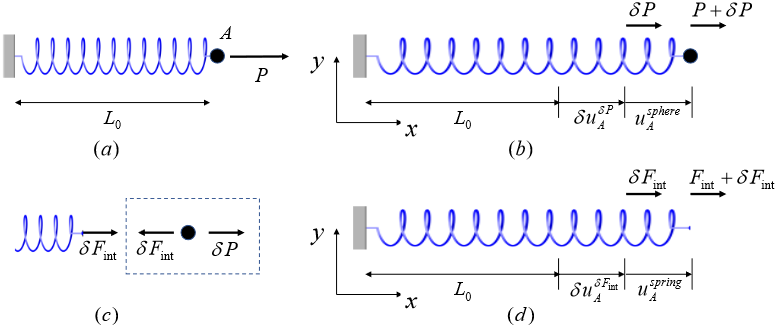
\includegraphics[width=0.666\linewidth]{Figures/Virtual_Force_Springs.png}\par
    $\delta W_e^* = u_A^{sphere} \delta P \rightarrow \delta F_{int}=\delta P$\par 
    $\delta W_e^* = -u_A^{spring} \delta F_{int}$\par 
    $\left(u_A^{sphere}-u_A^{spring}\right)\delta P=0$\par 
    This shows that the sum of the external and internal virtual work due to an 
    external virtual force (or moment) vanishes for structure in static 
    equilibrium, if the displacements and deformations are compatible.

    % ----- Virtual Force ----- %
    \textbf{Virtual Force Method for Computing Deflections}\par 
    $\delta W_e^*=u \delta P$ or $\delta W_E^* = \theta \delta M$ \par 
    Where $u$ is the real displacement of the point at which the virtual force
    is applied. \par 
    The internal virtual work can be written for a multi-component member as follows:\par 
    $\delta W_{ie}^*=\sum\limits_{N_m} \delta F_{int} \Delta$\par 
    Replace $\delta P$ with 1, $\bar{1}u=\sum\limits_N \bar{f}_{int}\Delta$

    % ----- Truss Example ----- %
    \textbf{Truss Example}
    
    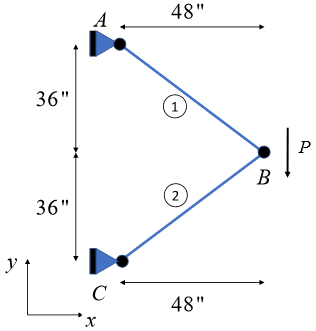
\includegraphics[width=0.5\linewidth]{Figures/Truss_Example_VF.png}

    $\delta W_{ie,bar}^*=\int_L \varepsilon \bar{\sigma} A dx\rightarrow 
    \delta W_{ie,bar}^*=\int_L \frac{\sigma}{E} \bar{\sigma} A dx$\par 
    For the case that the real and virtual stresses are constant in the bar, the 
    above expression can be expressed in terms of the real internal force, $N$, 
    and the virtual force, $\bar{n}$, as follows:\par 
    $\delta W_{ie,bar}^*=\frac{N\bar{n}L}{EA}$\par 
    For a truss composed of multiple bars:\par 
    $\delta W_{ie,truss}^* = \sum\limits_{i=1}^{N_b} \frac{N_i \bar{n}_i L_i}{E_i A_i}$\par 
    Using the balance of external and internal virtual work, i.e. $W_e^*=\delta 
    W_{ie,truss}^*$, and applying a dummy load in a particular direction, the 
    displacement, $d$, at the chosen joint in this direction can be computed by:\par 
    $\bar{1}d=\sum\limits_{i=1}^{N_b} \frac{N_i \bar{n}_i L_i}{E_i A_i}$\par
    Applying to example above:\par 
    \textbf{Step 1:} Compute internal forces, $N_i$, in the bars due to real load $P$. 
    Truss must be statically determinate.\par 
    $N_1=\frac{5}{6}P$ and $N_2=-\frac{5}{6}P$ \par 
    \textbf{Step 2:} Compute internal forces, $\bar{n}_i$, in the bars due to the 
    dummy loads $\bar{1}$. First, we apply a dummy load in the horizontal direction
    to compute the horizontal displacement.\par 
    $\bar{n}_1^u = \frac{5}{8}$ and $\bar{n}_2^u=\frac{5}{8}$ \par 
    Do the same for a vertical dummy load at joint B. \par 
    $\bar{n}_1^v = -\frac{5}{6}$ and $\bar{n}_2^v=\frac{5}{6}$\par 
    \textbf{Step 3:} To evaluate the internal work, summarize in a table: 
     
    \begin{center}
        \begin{tabular}{l|llllll}
            bar & $N_i$ & $\bar{n}_i^u$ & $\bar{n}_i^v$ & $A_i$ & $L_i$ & $E_i$ \\
            \hline
            1 & $\frac{5}{6}P$ & $\frac{5}{8}$ & $-\frac{5}{6}$ & $0.15$ & $60.0$ & $3\cdot 10^6$ \\
            $2$ & $-\frac{5}{6}P$ & $\frac{5}{8}$ & $\frac{5}{6}$ & $0.20$ & $60.0$ & $3\cdot 10^6$ \\
        \end{tabular}
    \end{center}

   \textbf{Step 4:} For each dummy load, evaluate the balance of external and 
   internal forces. \par 
   For the displacement in horizontal:\par 
   $\bar{1}u = \sum\limits_{i=1}^2 \frac{N_i\bar{n}_i^uL_i}{E_iA_i} = 8.33 \cdot 10^{-3} in$ \par 
   Vertical: \par 
   $\bar{1}v = \sum\limits_{i=1}^2 \frac{N_i\bar{n}_i^vL_i}{E_iA_i} = -44.4 \cdot 10^{-3} in$ \par

    % ----- Thermal Loading ----- %
    \textbf{Thermal Loading}
    Assuming that the material properties are constant in the bar and expressing
    the virtual stress in terms of the internal force, $\bar{n}$, we obtain:\par
    $\delta W_{ie,bar}^{*,thermal}=\alpha \Delta T \bar{n} L$\par 
    Defining an internal force due to differential heating/cooling as:\par
    $N^{thermal} = EA\alpha \Delta T$\par 
    we can write the internal virtual work by replacing the internal force due to
    mechanical loading, $N$, with one for thermal loading, $N^{thermal}$.\par 
    $\delta W_{ie,bar}^* = \frac{N^{thermal}\bar{n}L}{EA}$\par 
    From here follow same procedure as previous.

    % ----- Beam Example ----- %
    \textbf{Beam Example}\par 
    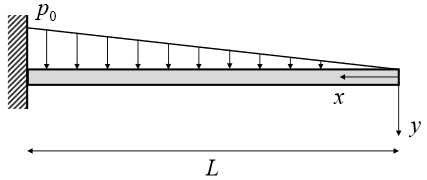
\includegraphics[width=0.5\linewidth]{Figures/Beam_Eample_VF.png}\par 
    First compute internal virtual work of the beam by virtual stress due to a unit dummy load.\par 
    $\delta W_{ie,beam}^*=\int \int \int_V \varepsilon\bar{\sigma}dxdydz$\par 
    Use Hook's Law: $\delta W_{ie,beam}^*=\int \int \int_V \frac{\sigma}{E}\bar{\sigma}dxdydz$\par 
    Recall: $\sigma = -\frac{M}{I}y$\par 
    Finally:\par 
    $\delta W_{ie,beam}^* = \int_L \frac{M\bar{m}}{EI}dx$ where $\bar{m}$ is
    virtual bending moment due to unit dummy load.

    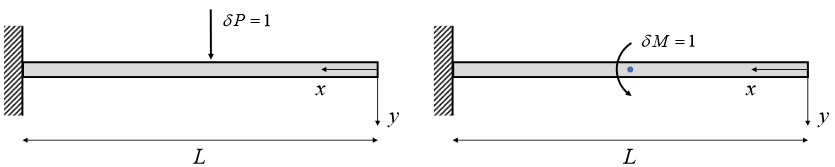
\includegraphics[width=\linewidth]{Figures/Beam_Eample_VF_2.png}\par 
    \textbf{Step 1:} Compute the bending moment due to the real force.\par 
    $M = \frac{p_0 x^3}{6L}$\par 
    \textbf{Step 2:} Compute bending moments due to unit dummy foce and unit
    dummy moment.\par 
    $\bar{m}^v=0$ for $0 \le x < \frac{L}{2}$ and $\bar{m}^v = x - \frac{L}{2}$
    for $\frac{L}{2} \le x \le L$\par 
    $\bar{m}^\phi = 0$ for $0 \le x < \frac{L}{2}$ and $\bar{m}^\phi = -1$
    for $\frac{L}{2} \le x \le L$\par
    \textbf{Step 3:} To compute the displacement and the rotation in the middle
    of the beam, compute the internal work due to the two dummy load cases.\par 
    $v\left(x=\frac{L}{2}\right) = \int_L \frac{M\bar{m}^v}{EI}dx=\int_{l/2}^L \frac{(x-\frac{L}{2})p_0x^3}{6EIL}dx$\par 
    $v\left(\frac{L}{2}\right) = \frac{49p_0L^4}{3840EI}$\par 
    Then do the same thing for $\phi$



\end{multicols*}  
\end{document}